\chapter{Resultados e Discussão}\label{cap:resultados}

Após entender o funcionamento do algoritmo de Viola Jones, foram executados testes com os conjuntos de imagens selecionados e os resultados obtidos são discutidos a seguir.

Inicialmente, foi necessário especificar com clareza como poderiam ser agrupadas as imagens, dada a sua origem e o resultado observado no teste, para isso foram utilizadas as definições da tabela \ref{grupos-images}. 

\begin{table}[htbp]
    \caption{Grupos observados}
    \label{grupos-images}
    \centering
    \begin{tabular}{ccc}\hline\hline
        \textbf{Grupo} & \textbf{Descrição} & \textbf{Quantidade} \\\hline
        \textit{A} & Imagens que não contêm nenhuma face & 17130 \\
        $\overline{A}$ & Imagens que contêm uma face & 17130 \\
        \textit{B} & Imagens onde o algoritmo não identificou nenhuma face & Variável \\
        $\overline{B}$ & Imagens onde o algoritmo identificou uma ou mais faces & Variável \\
    \hline\hline
    \end{tabular}
\end{table}

Definidos os grupos, pode-se utilizar uma tabela de contingência para facilitar o diagnóstico e discussão dos resultados obtidos.

\begin{table}[htbp]
    \caption{Tabela de contingência}
    \label{grupos-images}
    \centering
    \begin{tabular}{ccc}\hline\hline
        & \textit{B} & $\overline{B}$ \\
    \textit{A} & a (verdadeiro positivo) & b (falso negativo) \\
    $\overline{A}$ & c (falso positivo) & d (verdadeiro negativo) \\
    \hline\hline
    \end{tabular}
\end{table}

\begin{figure}[htb]
    \centering
    \caption{Possível distribuição normal dos grupos observados na tabela de contingência.}
    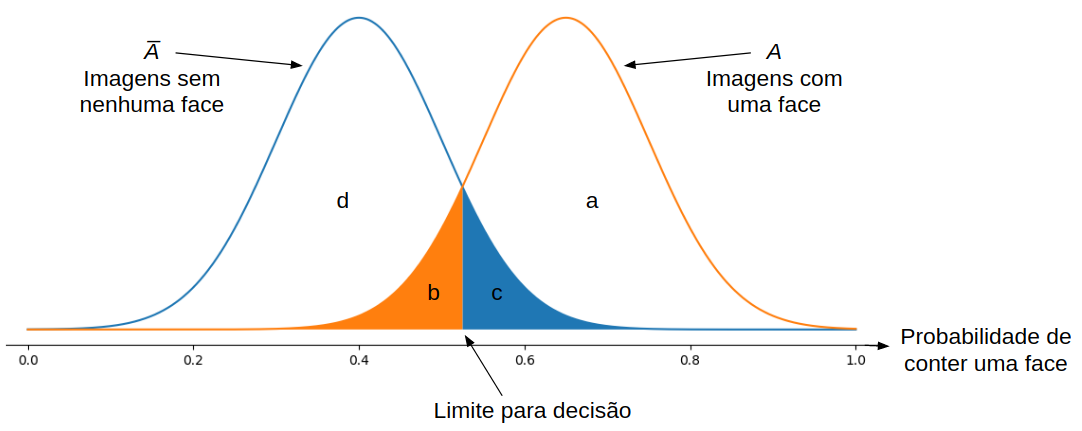
\includegraphics[scale=.5]{figs/norm_dist.png}
    \label{fig:norm_dist}
 \end{figure}

\begin{table}[htbp]
    \caption{Resultados Teste 3.}
    \label{resultados-teste-3}
    \begin{center}
    \begin{tabular}{rrr}\hline\hline
        \text{Número de faces} & \text{Número de imagens} & \text{Porcentagem} \\\hline
        0 & 263 & 1.5353\% \\
        1 & 8439 & 49.2645\% \\
        Mais de 1 & 8428 & 49.2002\% \\
    \hline\hline
    \end{tabular}
    \end{center}
\end{table}